\documentclass{beamer}
\usepackage[latin1]{inputenc}
\usetheme{Warsaw}
\usepackage{listings}
\usepackage{relsize}

\title{Port scans detector with prolog}
\author{Andrea Imparato - Lorenzo Tessari}\institute{Unversit\`a degli studi di Padova}

\begin{document}

\begin{frame}
\titlepage
\end{frame}



\begin{frame}
\frametitle{Cos'\`e?}
Software che riconosce la presenza 
di un port scanning su di un host in rete.\\

\textbf{Port scanning} = enumerazione porte attive/filtrate/chiuse\\[2cm]

2 tipologie di scanning:

\begin{itemize}

\item tcp scan

\item syn scan


\end{itemize}




\end{frame}



\begin{frame}
\frametitle{Motivazioni}
\begin{itemize}[<+->]
\item Tema sicurezza: conoscenza personale tool di sicurezza come \textbf{nmap} (port scanning) e \textbf{wireshark} (sniffing)
\item Snort IDS modulo port scanning non adeguato
\item Prolog!
\end{itemize}
\end{frame}


\begin{frame}
\frametitle{Use case}
 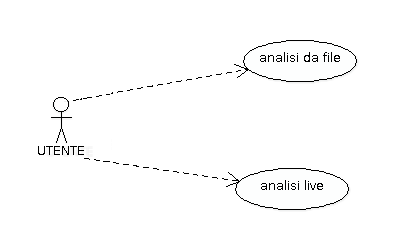
\includegraphics[width=10cm]{usecase1.png}
\end{frame}




\begin{frame}
\frametitle{Diagramma delle attivit\`a}
\begin{center}
 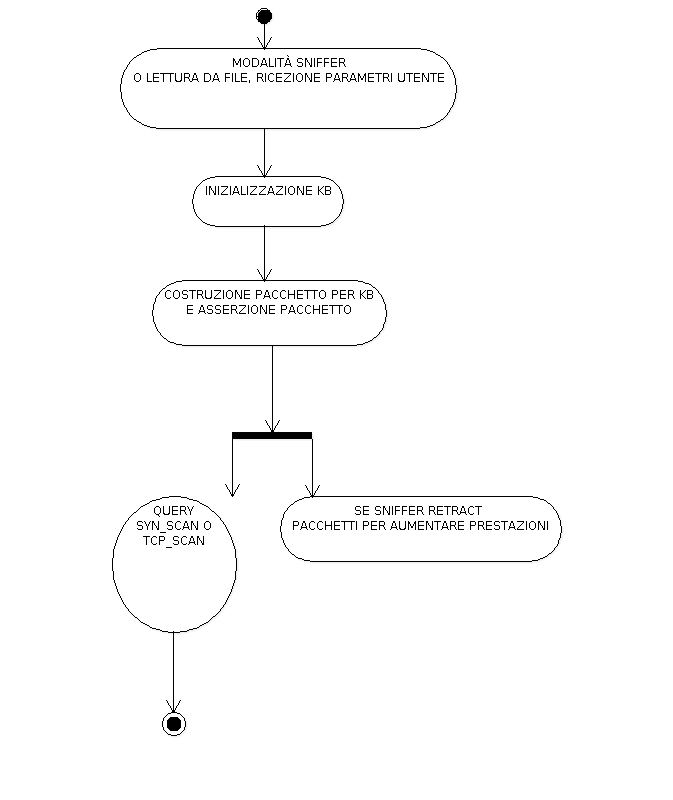
\includegraphics[height=8cm]{attivita.png}
\end{center}
\end{frame}



\begin{frame}
\frametitle{Progettazione}
Librerie:

\begin{itemize}
\item jpcap $\Rightarrow$ sniffer
\item tuprolog $\Rightarrow$ KB

\end{itemize}


\begin{center}
 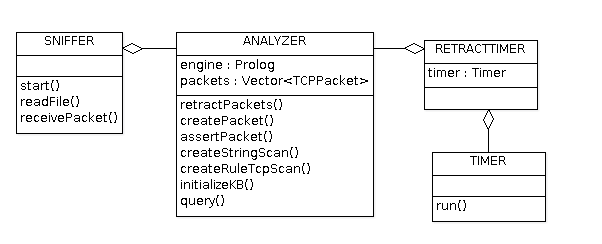
\includegraphics[height=5cm]{classi.png}
\end{center}
\end{frame}



\begin{frame}
\frametitle{Protocollo Tcp/Ip}
\begin{center}
 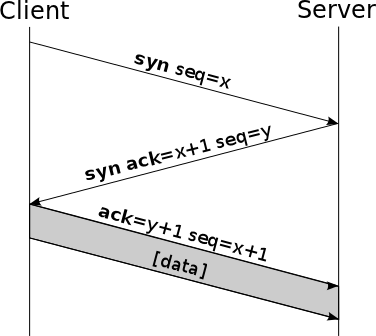
\includegraphics[width=5cm,height=5cm]{tcp.png}
\end{center}
\end{frame}



\begin{frame}[fragile]
\frametitle{Inferenza - Riconoscimento connessione tcp}
\begin{lstlisting}
/* regola per connessione tcp */
connessione_tcp(SOURCE,DESTINATION,SP,DP):-
pacchetto(SP,DP,syn,SOURCE,DESTINATION,X,0)
,pacchetto(DP,SP,syn,DESTINATION,SOURCE,Y,Z
,pacchetto(SP,DP,SOURCE,DESTINATION,Z,W)
,Z is X+1,W is Y+1.
\end{lstlisting}


\end{frame}


\begin{frame}[fragile]
\frametitle{Inferenza - Riconoscimento connessione syn}
\begin{lstlisting}
/* regola per connessione connessione syn */
connessione_syn(SOURCE,DESTINATION,SP,DP):-
pacchetto(SP,DP,syn,SOURCE,DESTINATION,X,0)
,pacchetto(DP,SP,syn,DESTINATION,SOURCE,Y,Z)
,Z is X+1.

\end{lstlisting}
\end{frame}



\begin{frame}[fragile]
\frametitle{Inferenza - Riconoscimento porta chiusa}
\begin{lstlisting}
/* regola per riconoscere se la porta e' chiusa */
porta_chiusa(SOURCE,DESTINATION,SP,DP):-
pacchetto(SP,DP,syn,SOURCE,DESTINATION,X,0)
,pacchetto(DP,SP,rst,DESTINATION,SOURCE,0,Z)
,Z is X+1.

\end{lstlisting}
\end{frame}


\begin{frame}[fragile]
\frametitle{Inferenza scan 4 porte}
\begin{lstlisting}
tcp_scan(X,Y):- 
connessione_tcp(X,Y,A1,A2),A1\=A2,
connessione_tcp(X,Y,A3,A4),
A3\=A4,connessione_tcp(X,Y,A5,A6)
,A5\=A6,connessione_tcp(X,Y,A7,A8)
,A7\=A8,A2\=A4,A2\=A6,A2\=A8,A4\=A6
,A4\=A8,A6\=A8.

syn_scan(X,Y):- 
connessione_syn(X,Y,A1,A2)
,A1\=A2,connessione_syn(X,Y,A3,A4),A3\=A4
,connessione_syn(X,Y,A5,A6),A5\=A6,
connessione_syn(X,Y,A7,A8),A7\=A8,A2\=A4,A2\=A6,
A2\=A8,A4\=A6,A4\=A8,A6\=A8.
\end{lstlisting}
\end{frame}


\begin{frame}
\frametitle{Risultati e sviluppi futuri}

\begin{itemize}[<+->]
\item In presenza di poco traffico sulla rete prestazioni ottime. Zero risultati di falsi positivi/negativi
sia per tcp scan sia syn scan.
\item Syn scan difficile da trovare con molto traffico. Euristiche nmap? 
\item Tcp scan quasi banale anche con molto traffico.
\item Implementazione IDS completo con tecniche di apprendimento automatico!
\end{itemize}

\end{frame}




\begin{frame}
\begin{center}
{\huge \textbf{DEMO!}}
\end{center}
\end{frame}




\end{document}
